\chapter*{Annexe B}\label{ch:annexeB}
\fancyhead[R]{\textit{Annexe B}}
\addcontentsline{toc}{part}{Annexe B}

 
 
 \subsection*{Cas d'utilisation « Consulter résumé de pointage des collaborateur »}
    Se cas est utilisé dans le bute d'avoir accès au informations de pointage des collaborateur, à partir d'une liste qui contiens le nom, prénom et le nom d'utilisateur ainsi que l'heure du dernier pointage et le statu de présence.
    
    Le manager pourras ensuite sélectionné un collaborateur pour avoir accès a la totalité de ses informations de pointage de manière détaillé.
        \begin{figure}[h!]
             \centering
            \includegraphics[scale=1.18]{images/DSS/DSS Consulter résumer de pointage des collaborateurs.png}
             \caption{Diagramme de séquence système « Consulter résumé de pointage des collaborateur »}
             \label{fig4}
        \end{figure}

    \subsection*{Cas d'utilisation « Consulter la liste des collaborateurs »}
    Un manager peut consulter la liste de ses collaborateurs (employés faisant partie d'une équipe dont il est responsable).A partir de cette liste il peux consulter le profil d'un collaborateur et avoir plus d'informations en cas de besoins.   
    
        \begin{figure}[h!]
             \centering
            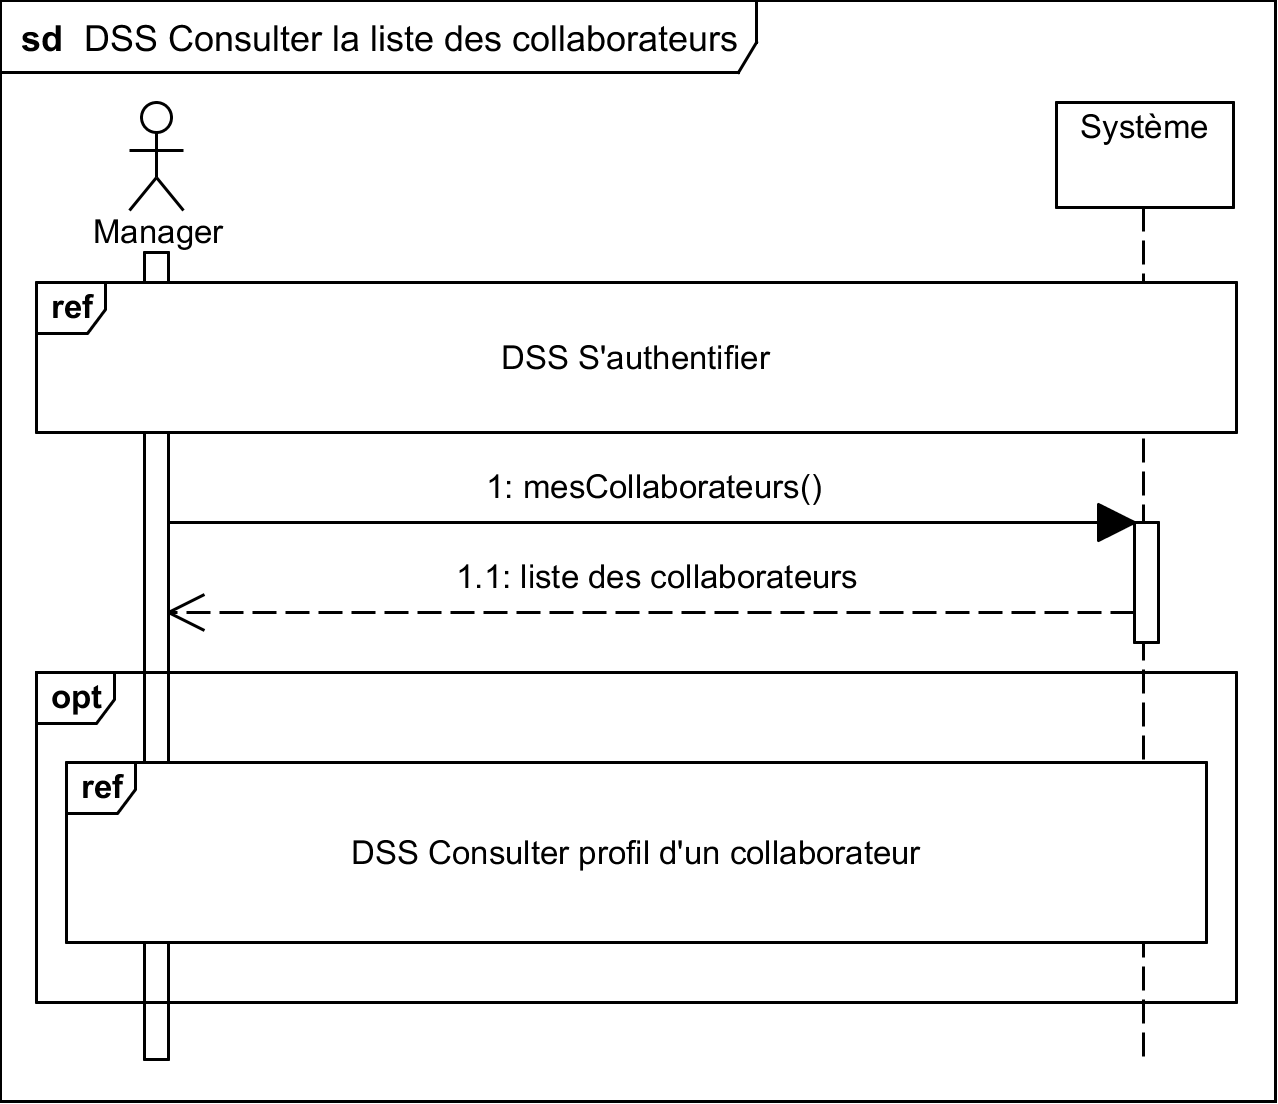
\includegraphics[scale=0.8]{images/DSS/DSS Consulter la liste des collaborateurs.png}
             \caption{Diagramme de séquence système « Consulter la liste des collaborateurs »}
             \label{fig4}
        \end{figure}
    
    \subsection*{Cas d'utilisation « Consulter mes équipes »}
    Un manager peut avoir une ou  plusieurs équipes,donc il aura besoin d'accéder à une liste de celles ci et accéder aux détails d'une équipe après l'avoir sélectionnée. 
        \begin{figure}[h!]
             \centering
            \includegraphics[scale=0.8]{images/DSS/DSS Consulter mes équipes.png}
             \caption{Diagramme de séquence système « Consulter mes équipes »}
             \label{fig4}
        \end{figure}
        \clearpage
        


    \subsection*{Cas d'utilisation « Consulter mon profil »}
    L'employé peux décider de consulter son profil et avoir accès au différentes informations qui les constitue en modifier certaines ou accéder a son planning. 
     
        \begin{figure}[h!]
             \centering
             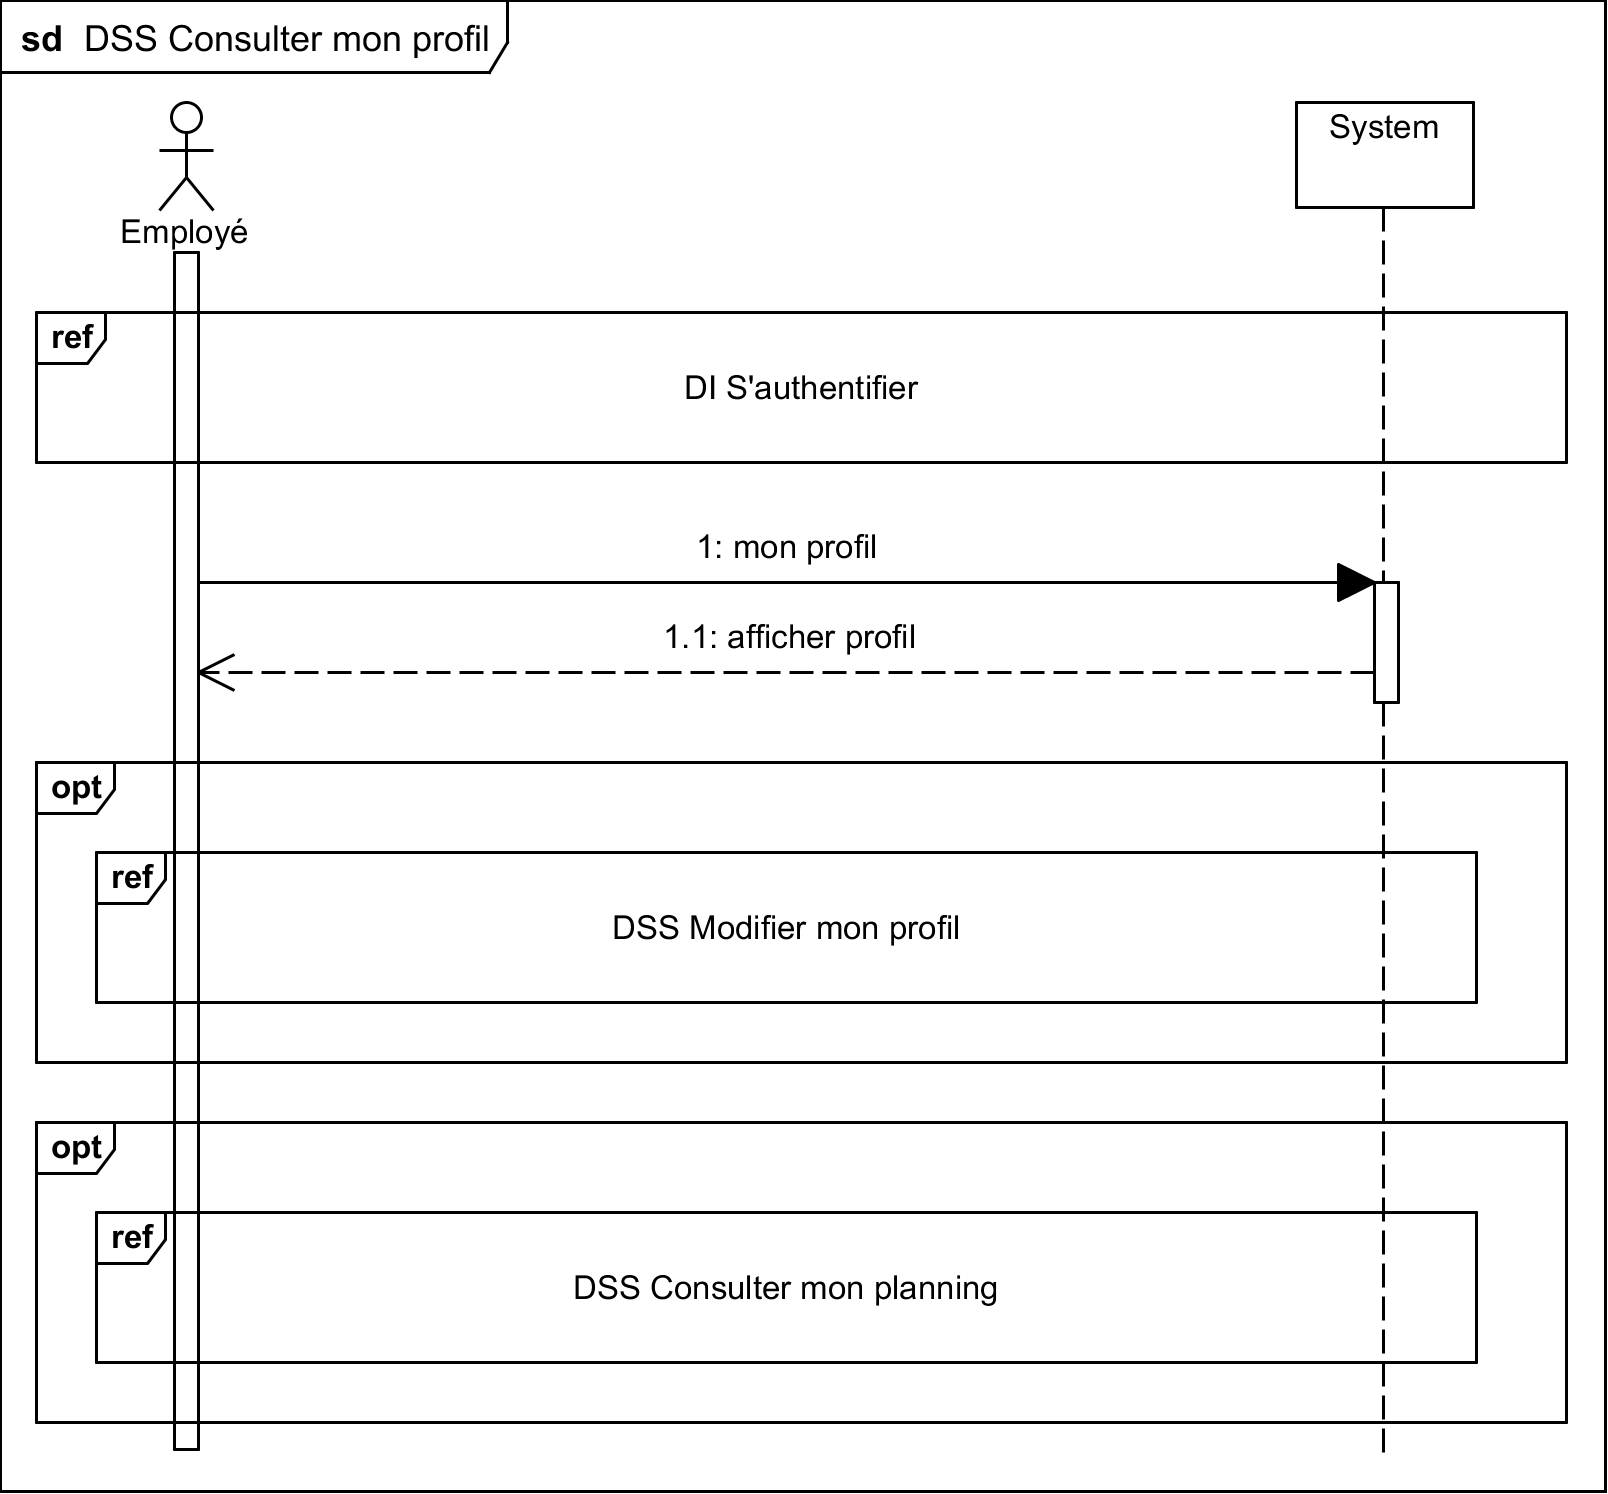
\includegraphics[scale=1]{images/DSS/DSS Consulter mon profil.png}
             \caption{Diagramme de séquence système « Consulter mon profil »}
             \label{fig4}
        \end{figure}
        
    \subsection*{Cas d'utilisation « Modifier mon profil »}
        Un employé peux modifier des informations de son profil sauf le nom,prénom et le nom d'utilisateur, qui sont définie par l'administrateur lors de l'enregistrement de l'employé en question de le système.
        \clearpage
        
        \begin{figure}[h!]
             \centering
             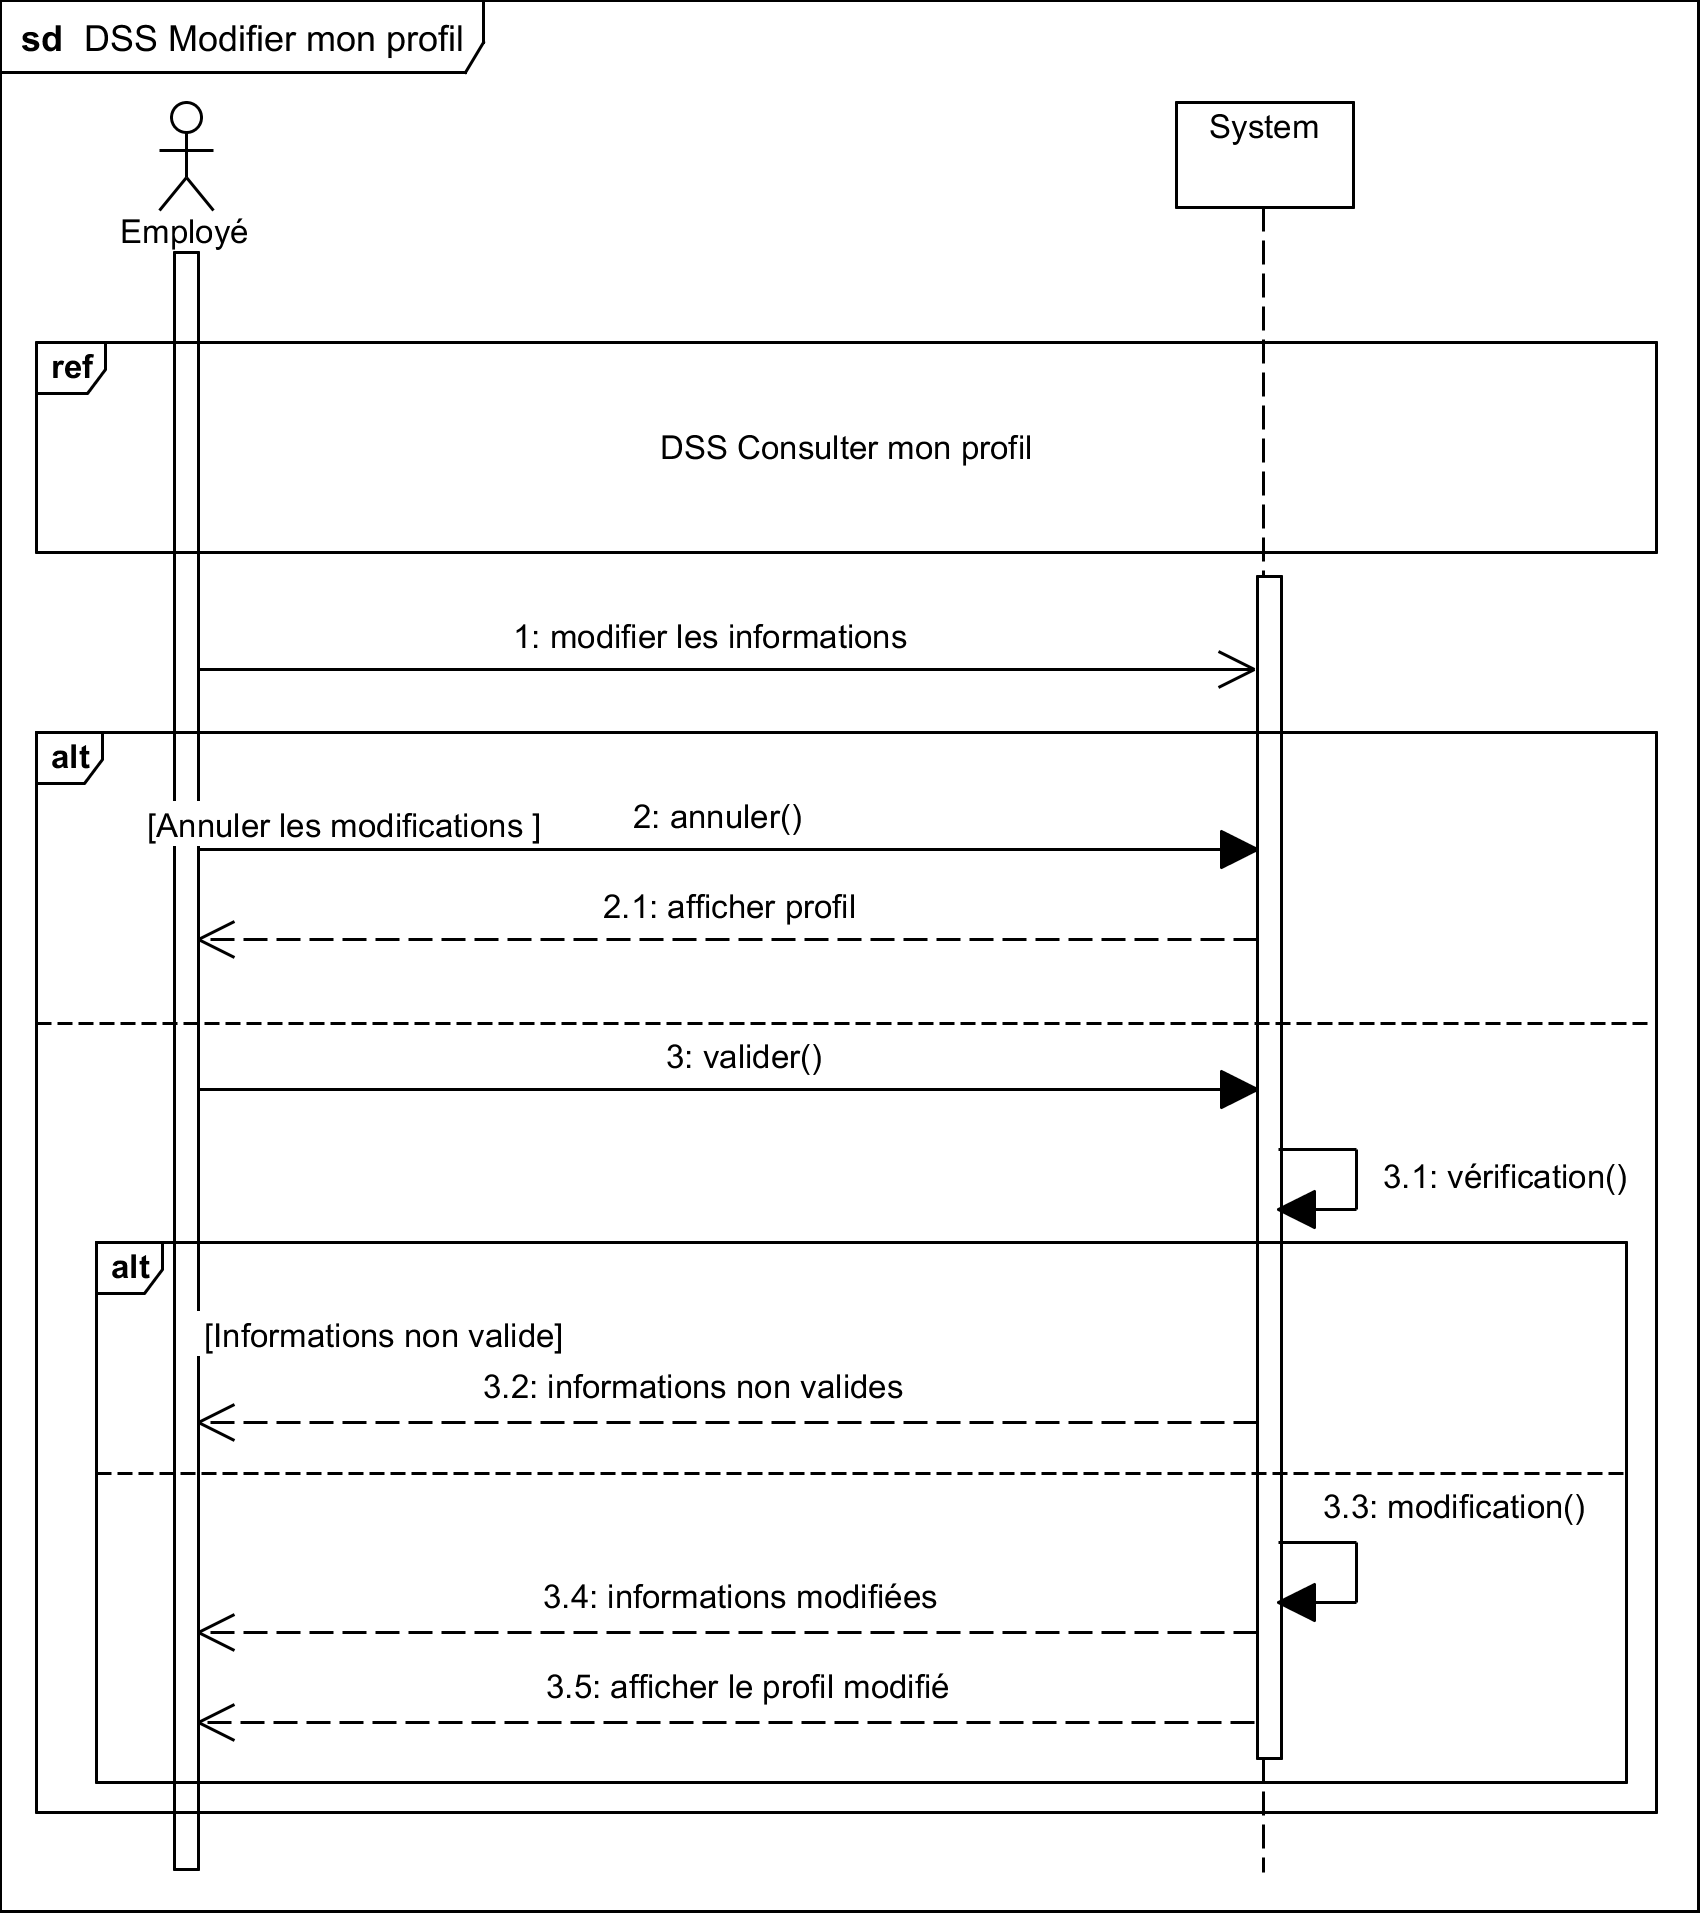
\includegraphics[scale=1]{images/DSS/DSS Modifier mon profil.png}
             \caption{Diagramme de séquence système « Modifier mon profil »}
             \label{fig4}
        \end{figure}


    \subsection*{Cas d'utilisation « Affectation d'un planning »}
    Le responsable a la possibilité d'affecter des plannings a tous les employés. Une fois le planning créé il peut l'attribuer a des employés pour que ils soient au courant  des horaires de travail.  
    \clearpage
        \begin{figure}[h!]
             \centering
            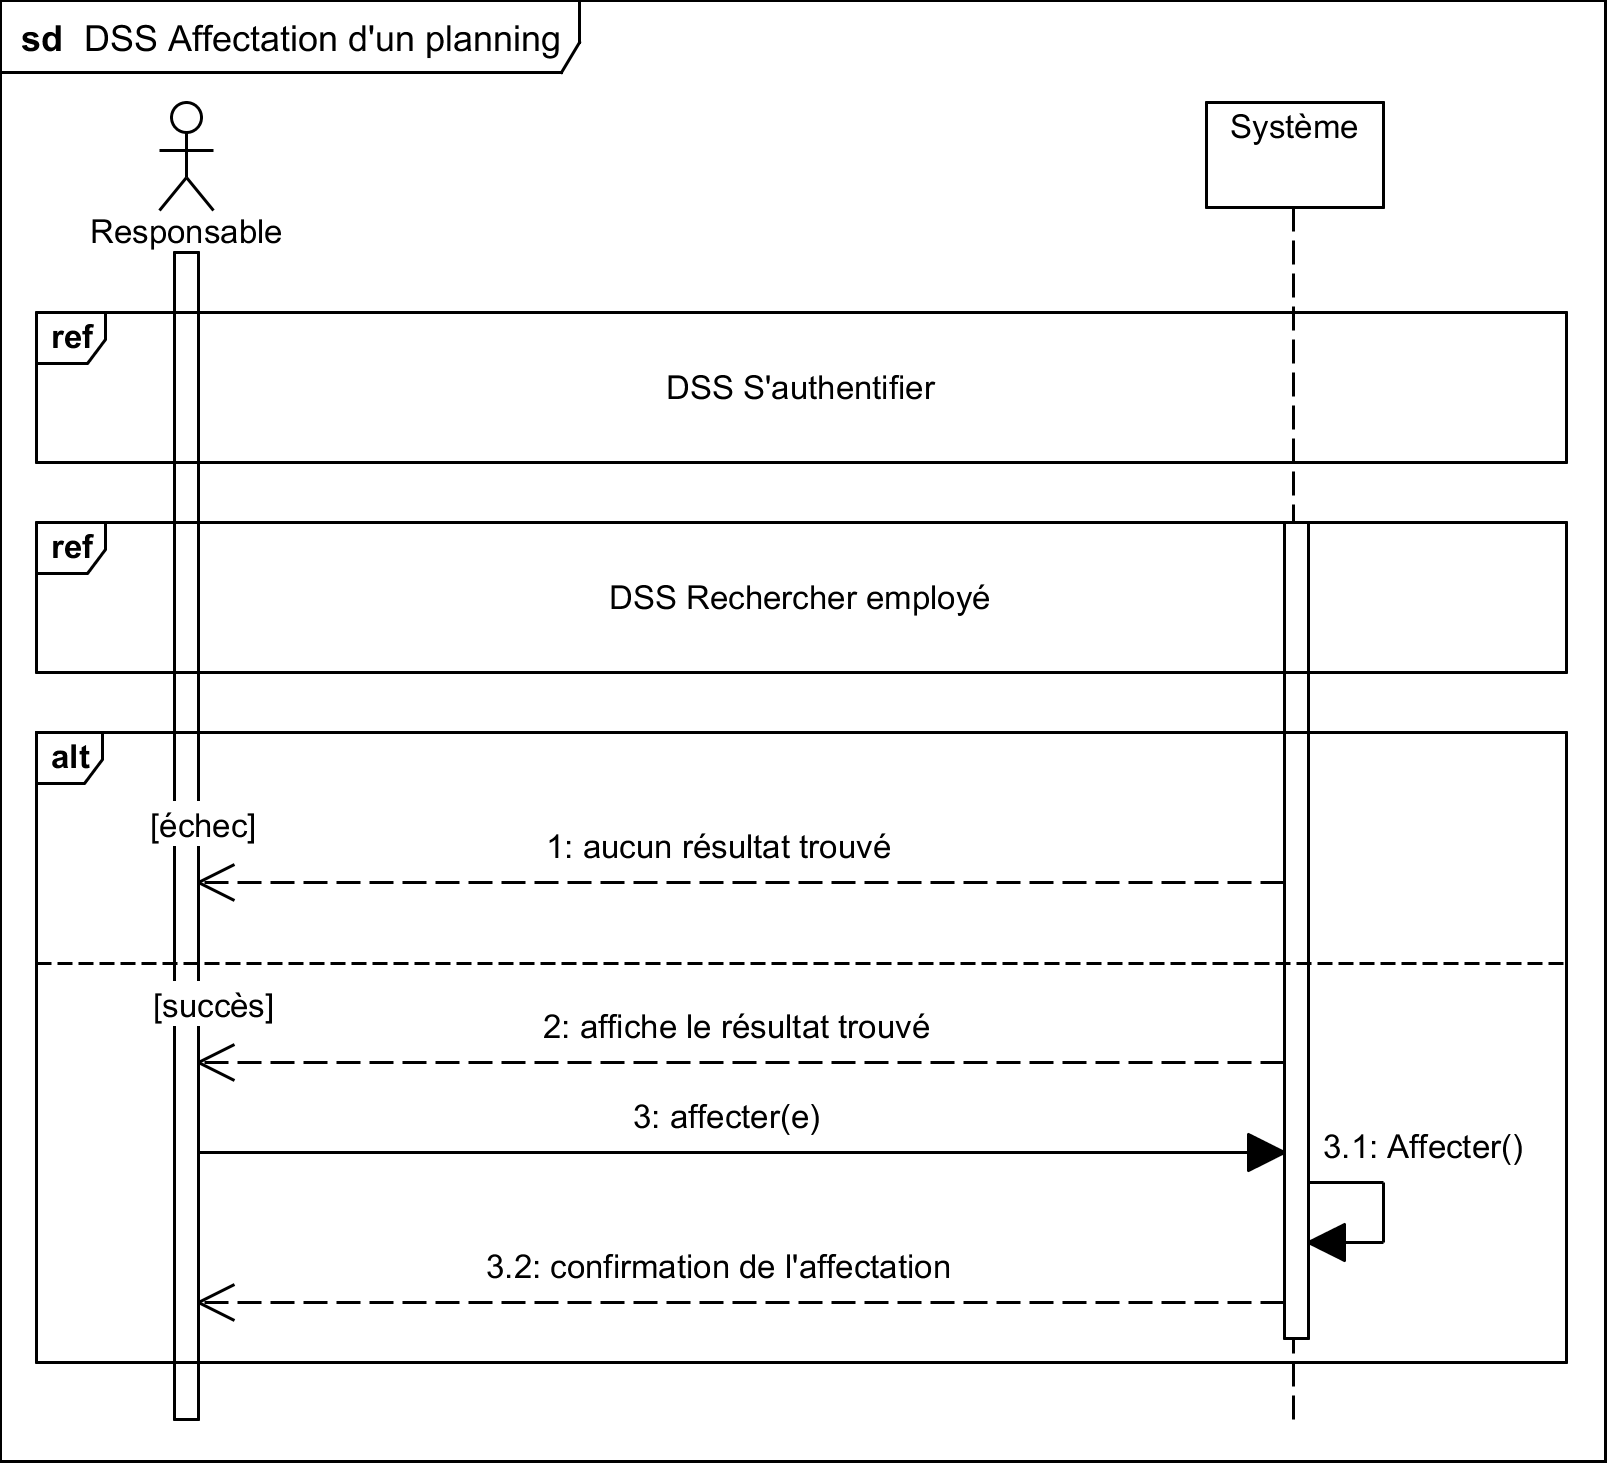
\includegraphics[scale=0.85]{images/DSS/DSS Affectation d'un planning.png}
             \caption{Diagramme de séquence système « Affectation d'un planning »}
             \label{fig4}
        \end{figure}
    
    
    
    
    \subsection*{Cas d'utilisation « Consulter liste des équipes »}
    Grâce a ce cas une responsable consulte la liste des équipes existantes avec l'intitulé et le nom,prénom du manager de chaque équipe.A partir de cette liste il peut gérer les équipes ou consulter les informations détaillées à-propos d'une équipe une fois sélectionnée.  
    \clearpage
        \begin{figure}[h!]
             \centering
            \includegraphics[scale=1.2]{images/DSS/DSS Consulter liste des équipes.png}
             \caption{Diagramme de séquence système « Consulter liste des équipes »}
             \label{fig4}
        \end{figure}
        
    \subsection*{Cas d'utilisation « Ajouter empreinte »}
    Lorsque un employé intègre l'entreprise.l'administrateur lui crée un compte dans le système et saisit les informations principales pour ensuite ajouter son empreinte dans la pointeuse.Une opération décrite dans ce cas d'utilisation.En premier lieu il active le mode enregistrement de la pointeuse et demande a l'employé de posé son index droit une premier fois le retire et le place de nouveau pour confirmation.Une fois l'empreinte enregistrée l'administrateur est notifier du bon déroulement de l'opération.    
    \clearpage
        \begin{figure}[h!]
             \centering
            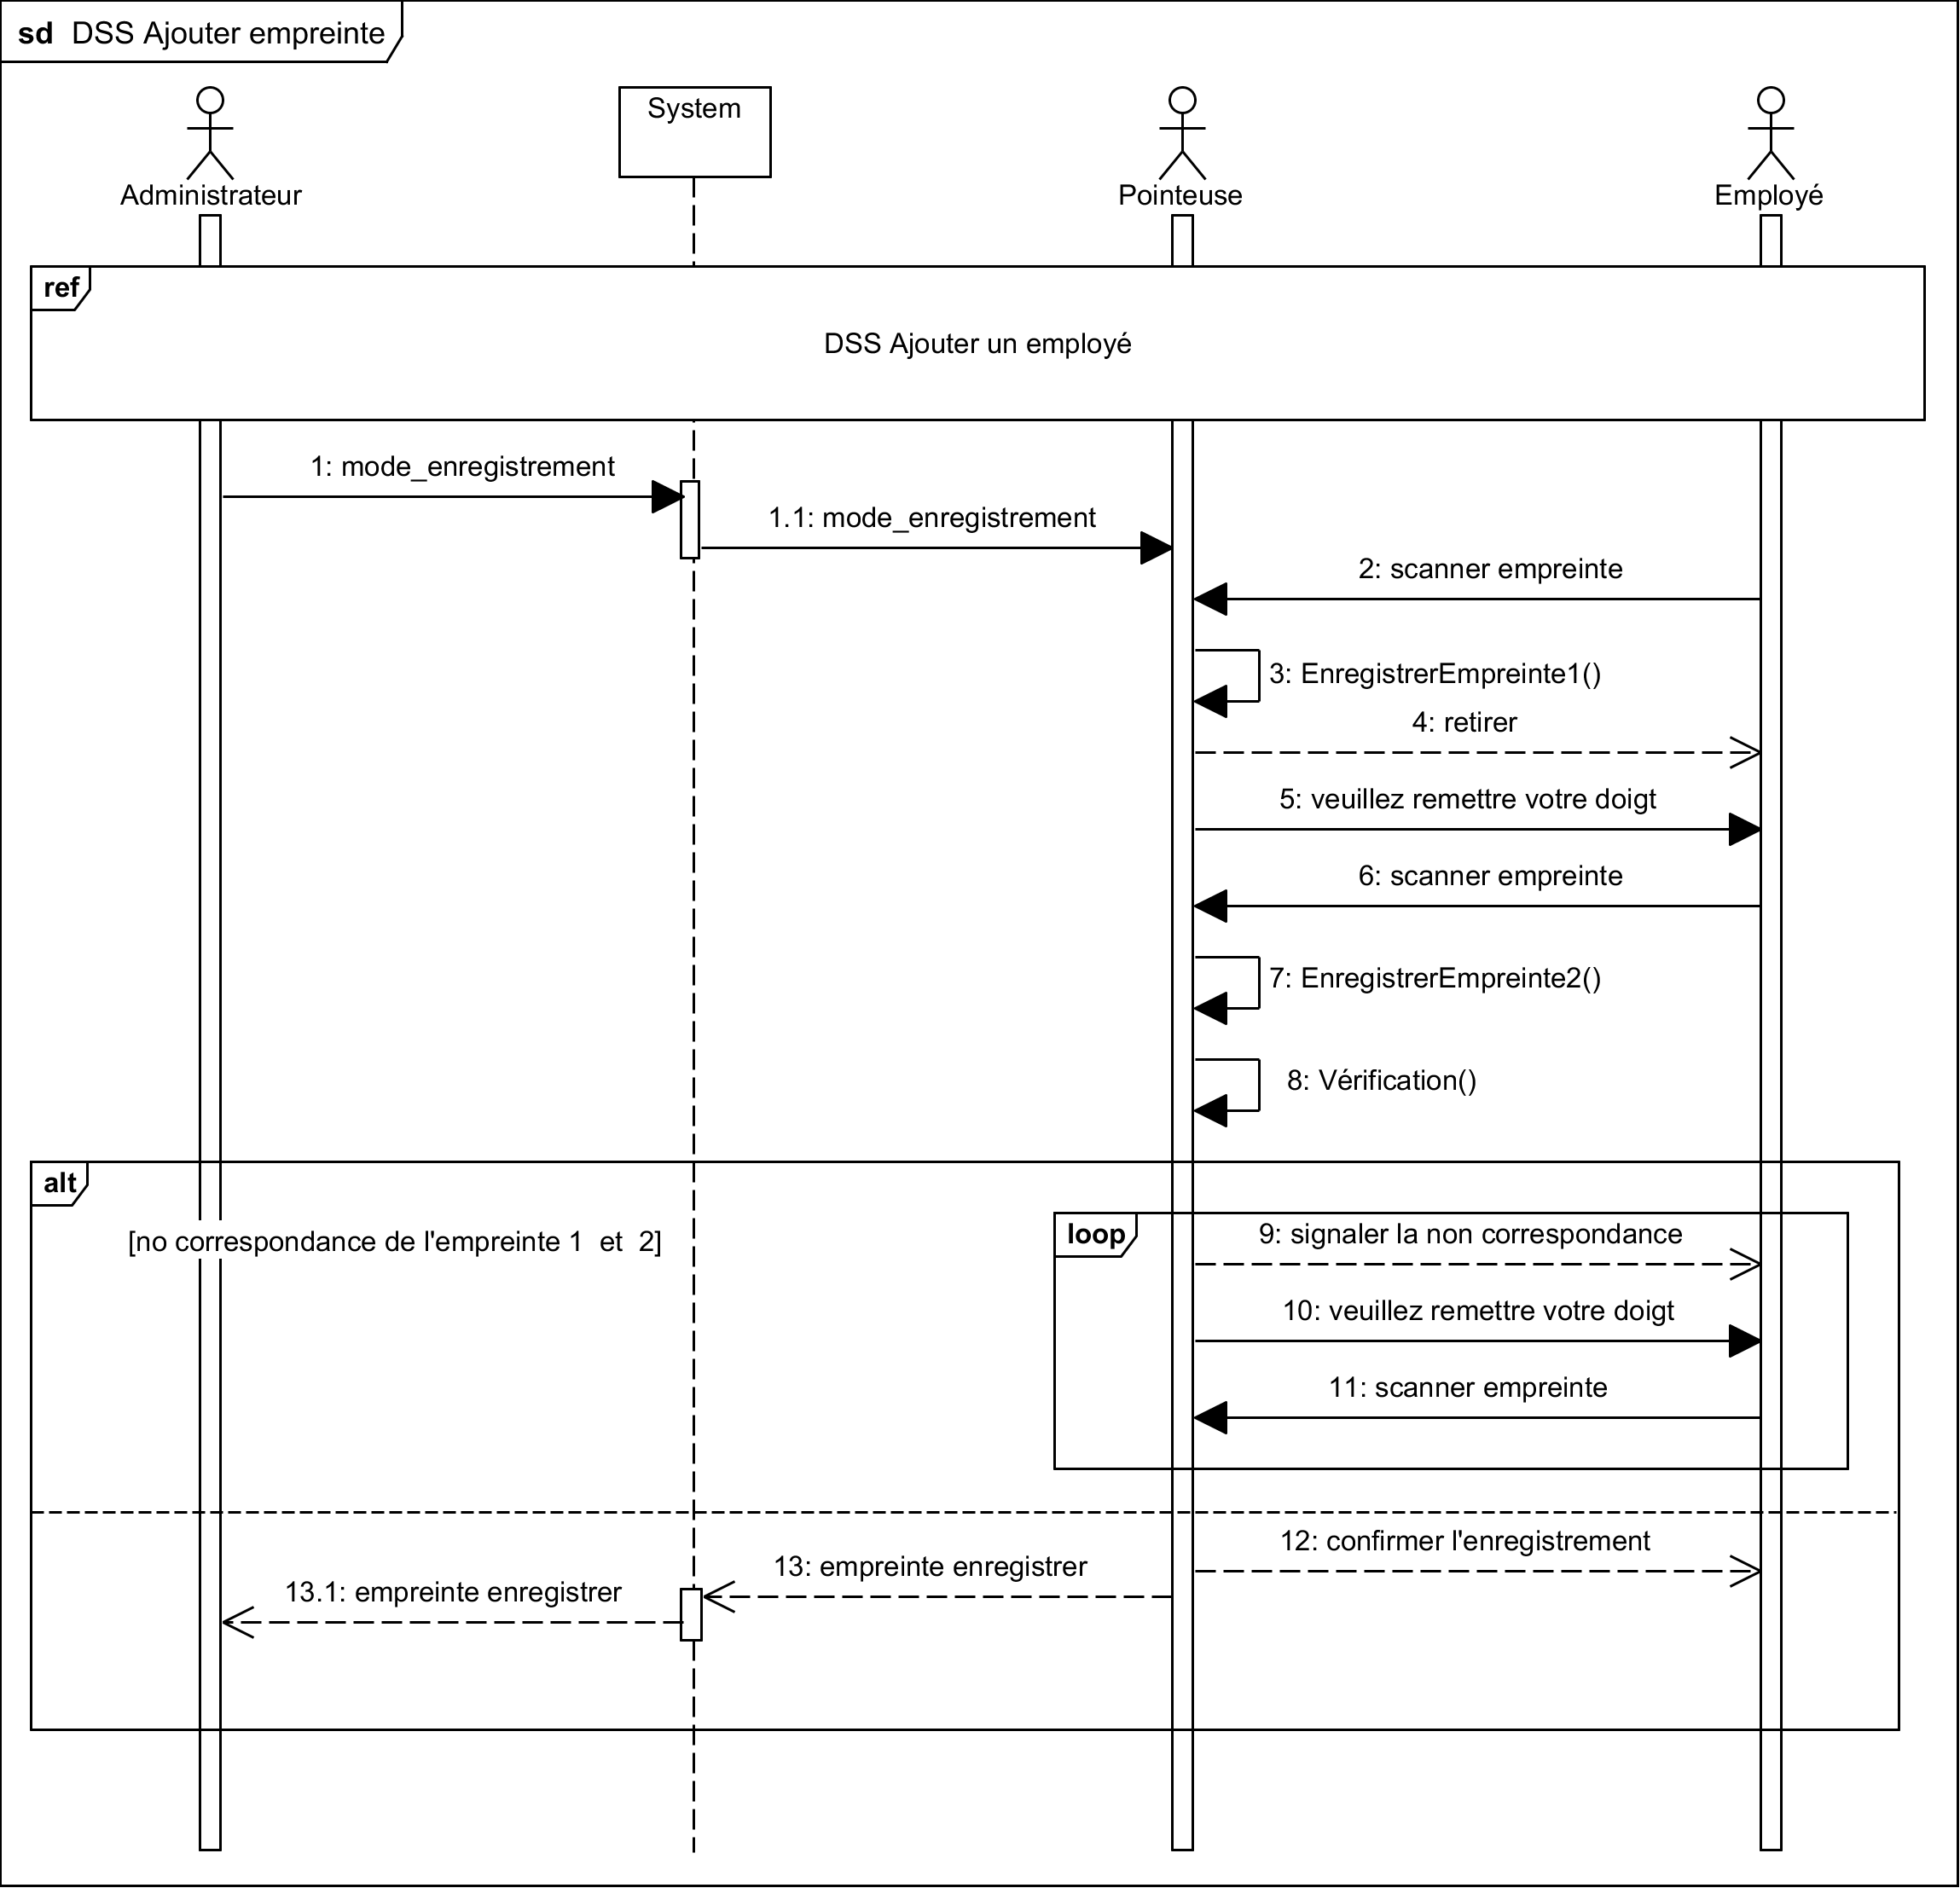
\includegraphics[scale=0.85,angle=90]{images/DSS/DSS Ajouter empreinte.png}
             \caption{Diagramme de séquence système « Ajouter empreinte »}
             \label{fig4}
        \end{figure}
        
    \subsection*{Cas d'utilisation « Supprimer empreinte »}
    Ce cas d'utilisation est déclenché lorsque l'administrateur supprime un employé. La pointeuse passe en mode suppression et récupère l'identifiant de l'empreinte a supprimé puis la supprime en confirmant la suppression au système qui confirme la suppression au responsable a son tour.
    \clearpage
        \begin{figure}[h!]
             \centering
            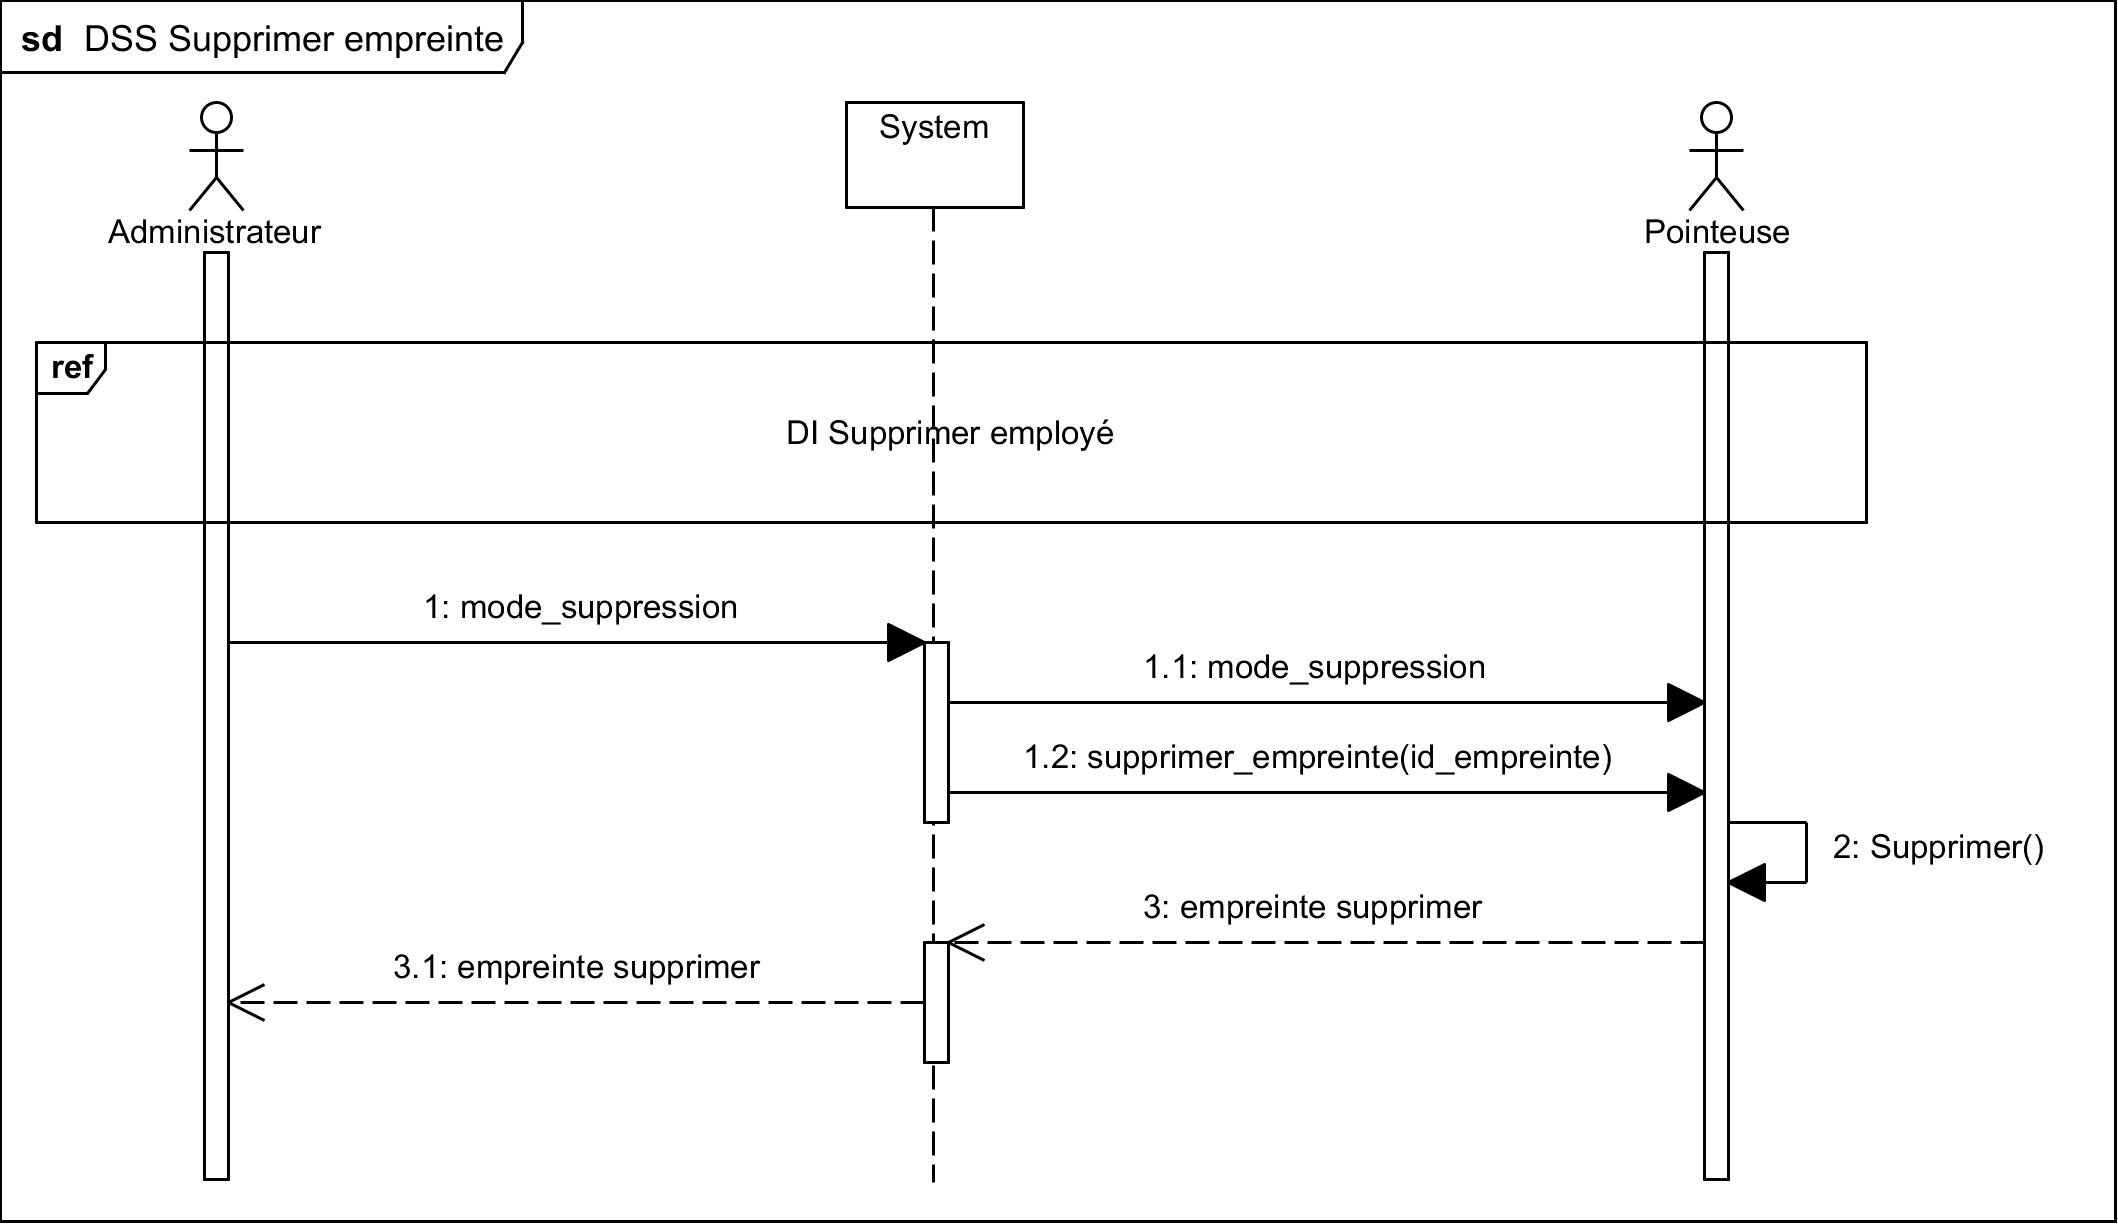
\includegraphics[scale=0.95]{images/DSS/DSS Supprimer empreinte.png}
             \caption{Diagramme de séquence système « Supprimer empreinte »}
             \label{fig4}
        \end{figure}
    
    \clearpage